\documentclass[conference]{IEEEtran}
\usepackage{cite}
\usepackage{booktabs}
\usepackage{tabularx}
\usepackage{array}
\usepackage{url}
\usepackage{microtype}
\usepackage{tikz}
\usepackage{dblfloatfix}
\usetikzlibrary{arrows.meta,positioning,shapes.geometric}
\newcolumntype{Y}{>{\raggedright\arraybackslash}X}
\emergencystretch=1.5em
\raggedbottom
\title{AI-Driven Cybersecurity Threat Detection and Automated Response:\\A Review of Machine Learning, Deep Learning, Anomaly Detection, and Generative AI}
\author{
\IEEEauthorblockN{Satyajeet Kumar}
\IEEEauthorblockA{Department of Computer Science \& Engineering\\
Sharda School of Computing Science \& Engineering\\
Sharda University, Greater Noida, India\\
satyajeetzod@gmail.com}
\and
\IEEEauthorblockN{Ashish Shakya}
\IEEEauthorblockA{Department of Computer Science \& Engineering\\
Sharda School of Computing Science \& Engineering\\
Sharda University, Greater Noida, India\\
ashishrahin@gmail.com}
\and
\IEEEauthorblockN{Ritanshu Kumar}
\IEEEauthorblockA{Department of Computer Science \& Engineering\\
Sharda School of Computing Science \& Engineering\\
Sharda University, Greater Noida, India\\
2023216269.ritanshu@ug.sharda.ac.in}
\and
\IEEEauthorblockN{Swati Singal}
\IEEEauthorblockA{Department of Computer Science \& Engineering\\
Sharda School of Computing Science \& Engineering\\
Sharda University, Greater Noida, India\\
swati.singal@sharda.ac.in}
\and
\IEEEauthorblockN{Mayank Kumar Goyal}
\IEEEauthorblockA{Department of Computer Science \& Engineering\\
Sharda School of Computing Science \& Engineering\\
Sharda University, Greater Noida, India\\
mayank.goyal2@sharda.ac.in}}
\begin{document}
\maketitle
\begin{abstract}
Cybersecurity detection is no longer a choice between a fixed signature database and a single machine-learning classifier. In practice, security teams combine rules, behavioral signals, threat intelligence, and analyst judgment, often under severe time pressure. This review examines that combination across intrusion detection, malware and phishing analysis, anomaly detection, explainable AI, generative AI, retrieval-augmented generation (RAG), and automated response. The eleven supplied studies are read alongside verified external research and compared by evidence, data, evaluation design, and limitation. Reported evaluation measures include accuracy, precision, recall, F1-score, AUC-ROC, false-positive rate, and response latency, although the availability of each metric differs across studies. The comparison suggests that signatures and rules remain dependable for known indicators, while learned models extend visibility into relationships and deviations that are difficult to encode manually. It also shows why impressive accuracy values should be treated cautiously when datasets are imbalanced, temporally leaky, or far removed from operational traffic. Generative models may reduce the burden of intelligence synthesis, but they add risks involving hallucination, provenance, prompt injection, privacy, and unsafe automation. The resulting argument is for an evidence-linked, human-supervised architecture rather than unrestricted autonomy. SecureX is mentioned only as a possible framework motivated by these findings, not as a validated experimental system.
\end{abstract}
\begin{IEEEkeywords}
cybersecurity, intrusion detection, anomaly detection, machine learning, deep learning, explainable AI, large language models, retrieval-augmented generation, automated incident response, security operations center
\end{IEEEkeywords}

\section{Introduction}
Security operations centers (SOCs) work with a messy mixture of network events, endpoint telemetry, vulnerability advisories, malware reports, identity signals, and analyst observations. These sources arrive at different speeds and rarely agree perfectly. The practical challenge is therefore broader than classifying an event as benign or malicious. A useful system must recognize known indicators, notice unfamiliar behavior, estimate operational risk, explain the basis of an alert, and recommend a response that does not create a second incident. The supplied literature captures this wider problem through a CERT threat observatory \cite{Kaufhold2022}, deep-learning and anomaly-detection studies \cite{Rajendran2024}, text-mining risk assessment \cite{KumarBhatRisk}, temporal threat intelligence \cite{KumarBhatTemporal}, and AI-assisted advisory workflows \cite{Abeywardena2023,Ismail2024,Zhivonitko2026}.

Traditional signatures and rules still earn their place in this environment. They are fast, auditable, and effective when the indicator or behavior is already understood. Their weakness is equally clear: knowledge that has not been encoded cannot be detected by the rule itself. Statistical and machine-learning methods offer broader pattern recognition, but their apparent accuracy can fall sharply when traffic changes or when training and test data are not operationally independent \cite{SommerPaxson,BuczakGuven,Liao2013,Arp2022}. Deep models can learn useful representations from sequences, graphs, and binary artifacts, although they bring additional data, computational, and explanation costs \cite{Shone2018}. Generative AI may help analysts organize large volumes of intelligence, but fluent language is not the same thing as reliable security evidence \cite{Lewis2020,Liu2025}.

The review consequently focuses on four connected questions: where known-threat detection ends and unknown-threat discovery begins; what the literature actually demonstrates about hybrid and real-time systems; how explainability, LLMs, and RAG can assist analysis without weakening provenance; and which limitations are strong enough to define credible research gaps. This is a review paper, not an implementation report. SecureX is therefore used only as a possible direction suggested by the literature, and no accuracy, detection rate, or response-performance claim is attributed to it.

\section{Review Scope and Source Treatment}
The eleven supplied PDFs form the core of the review. Each was read for its research problem, method, data source, evaluation evidence, limitation, and stated future work. External studies were added only where the supplied set left a clear gap, particularly around foundational IDS limitations, benchmark datasets, online anomaly detection, adversarial robustness, model explanation, and RAG. When a paper did not provide enough reliable information, the tables say ``Not reported'' rather than filling the gap with an assumption.

The source set is heterogeneous. Kaufhold \emph{et al.} present a design-science dashboard evaluated with expert walkthroughs and interviews rather than a detection-accuracy benchmark \cite{Kaufhold2022}. The supplied deep-learning study reports CNN and RNN results but gives limited information in its abstract about dataset construction and external validation \cite{Rajendran2024}. The text-mining risk-assessment study reports XGBoost, random forest, SVM, logistic regression, and autoencoder components \cite{KumarBhatRisk}. The GNN/LLM study combines file fingerprints, graph convolution, LIME, and language-model context, but its result is evidence about a proposed system rather than proof of general deployment performance \cite{Balaji2025}.

\begin{table*}[t]
\caption{AI Models, Techniques, Tasks, and Dataset Evidence}
\label{tab:models}
\centering\scriptsize
\begin{tabularx}{\textwidth}{c Y Y Y Y Y}
\toprule
Ref. & AI model or technique & Security task & Dataset or data source & Reported metrics & Review interpretation\\
\midrule
\cite{Kaufhold2022} & Dashboard algorithms, filtering, source interrelations & CERT situational awareness & Public cyber-information sources; exact corpus not reported & 12 expert walkthrough/interviews & Operational usability study, not classifier validation\\
\cite{Manoharan2022} & ML, deep learning, NLP, behavioral analysis & General threat detection and response & Literature and case material & Review evidence; no common benchmark & Taxonomy and challenge discussion\\
\cite{Abeywardena2023} & NLP, threat-feed processing, dashboard generation & SOC advisory reports & Threat databases and RSS feeds & Metrics not reported in supplied paper & Workflow automation proposal\\
\cite{Rajendran2024} & CNN, RNN, anomaly detection & Intrusion and zero-day-oriented detection & Dataset name not reported in abstract & Accuracy: CNN 93\%, RNN 96\%; precision, recall, F1, AUC-ROC, FPR, and latency: Not reported & Results require dataset and split details\\
\cite{KumarBhatRisk} & TF-IDF, embeddings, CVSS features, XGBoost, RF, SVM, LR, autoencoder & Vulnerability risk classification and novelty detection & Security bulletins and advisory data & Accuracy: 92\%; precision: 0.91; recall: 0.94; AUC-ROC: 0.95; F1, FPR, and latency: Not reported & Text-risk assessment with incomplete external validation\\
\cite{Balaji2025} & GCN, locality-sensitive hashing, LIME, LLM context & File and malicious-behavior detection & Uploaded files; exact public dataset not reported & Model evaluation described; comparable metrics not available in abstract & Explainability-oriented prototype\\
\cite{Liu2025} & LLM, specialized NLP modules, agentic CTI & Attribution, contextualization, prioritization, remediation support & 271,570 threat reports & Comparative evaluation against LLMs and agents & Strong information-integration direction; safety remains open\\
\cite{Zhivonitko2026} & Open conversational models and LoRA fine-tuning & Conversational cyber-threat advising & Curated cybersecurity question-answer data & Automatic metrics; exact values not used here & Domain adaptation study, not an operational SOC trial\\
\cite{SommerPaxson} & Supervised ML for NIDS, methodological analysis & Network intrusion detection & Operational network data assumptions & Analytical critique of closed-world evaluation & Establishes generalization risk\\
\cite{Mirsky2018} & Ensemble of autoencoders and online feature mapping & Streaming network anomaly detection & Network streams and testbed traffic & Online detection evaluation; deployment-specific & Supports real-time anomaly architecture\\
\cite{Shone2018} & Deep autoencoder and supervised classifier & Network intrusion detection & Benchmark network traffic; study-specific & Benchmark evaluation; cross-domain limits remain & Deep representation learning evidence\\
\cite{Lewis2020} & Dense retrieval plus sequence-to-sequence generation & Knowledge-intensive question answering & Wikipedia index in original study & Multiple open-domain QA tasks & RAG foundation, not security validation\\
\bottomrule
\end{tabularx}
\end{table*}

\begin{figure*}[!t]
\centering
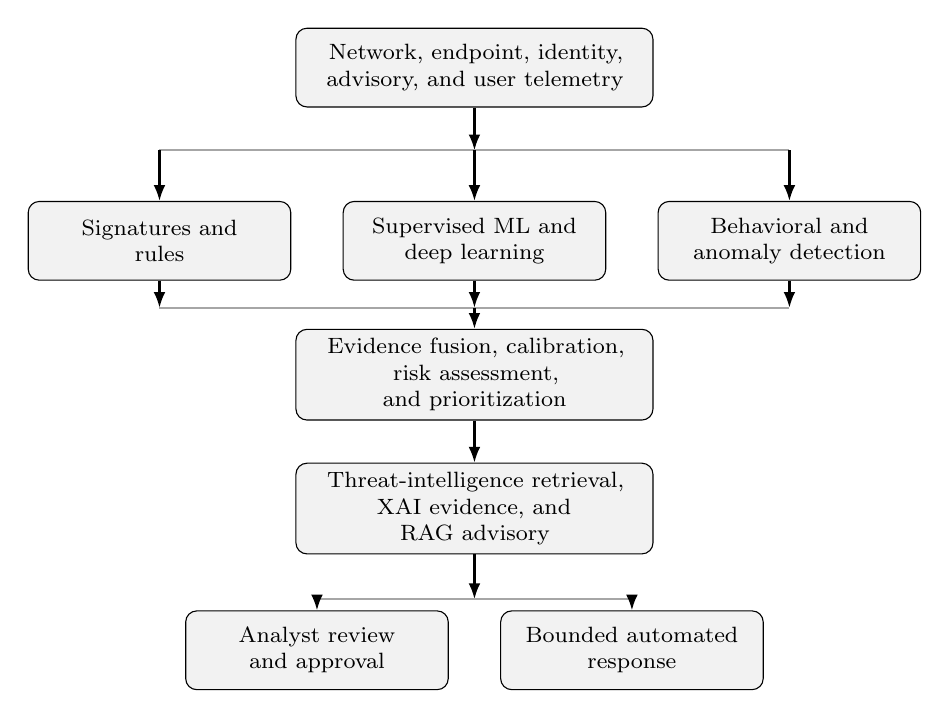
\begin{tikzpicture}[every node/.style={font=\footnotesize}, box/.style={draw, fill=gray!10, rounded corners, align=center, minimum height=10mm, text width=31mm}, wide/.style={draw, fill=gray!10, rounded corners, align=center, minimum height=10mm, text width=43mm}, arrow/.style={-{Latex[length=2mm]}, thick}]
\node[wide] (telemetry) at (0,4.4) {Network, endpoint, identity,\\advisory, and user telemetry};
\node[box] (det) at (-4,2.2) {Signatures and\\rules};
\node[box] (ml) at (0,2.2) {Supervised ML and\\deep learning};
\node[box] (anom) at (4,2.2) {Behavioral and\\anomaly detection};
\node[wide] (fusion) at (0,0.5) {Evidence fusion, calibration,\\risk assessment, and prioritization};
\node[wide] (context) at (0,-1.2) {Threat-intelligence retrieval,\\XAI evidence, and RAG advisory};
\node[box] (human) at (-2,-3.0) {Analyst review\\and approval};
\node[box] (auto) at (2,-3.0) {Bounded automated\\response};
\coordinate (bus) at (0,3.35);
\draw[arrow] (telemetry.south) -- (bus);
\draw[gray!70, thick] (-4,3.35) -- (4,3.35);
\draw[arrow] (-4,3.35) -- (det.north);
\draw[arrow] (0,3.35) -- (ml.north);
\draw[arrow] (4,3.35) -- (anom.north);
\draw[gray!70, thick] (-4,1.35) -- (4,1.35);
\draw[arrow] (det.south) -- (-4,1.35);
\draw[arrow] (ml.south) -- (0,1.35);
\draw[arrow] (anom.south) -- (4,1.35);
\draw[arrow] (0,1.35) -- (fusion.north);
\draw[arrow] (fusion.south) -- (context.north);
\draw[arrow] (context.south) -- (0,-2.35);
\draw[gray!70, thick] (-2,-2.35) -- (2,-2.35);
\draw[arrow] (-2,-2.35) -- (human.north);
\draw[arrow] (2,-2.35) -- (auto.north);
\end{tikzpicture}
\caption{Evidence-preserving hybrid detection and response architecture synthesized from the reviewed literature. Feedback, rollback, and audit controls are discussed in the text; the diagram is conceptual and does not claim SecureX implementation results.}
\label{fig:architecture}
\end{figure*}

\section{Detection Paradigms}
\subsection{Signature and Rule-Based Detection}
Signature detection maps an event to a known pattern such as a hash, byte sequence, domain, IP address, or malware rule. Rule-based systems extend this idea with expert-defined conditions over events, identities, sequences, and context. Both provide low-latency decisions and useful audit trails. They are appropriate for confirmed malware families, known phishing infrastructure, policy violations, and high-confidence containment triggers. Their weakness is brittleness: a small artifact change can evade a signature, while an overly broad rule creates false positives. Signatures encode historical knowledge and cannot independently discover a genuinely novel attack.

The literature does not support replacing deterministic controls with learned models. It supports layered detection. A signature can establish high-confidence evidence; a rule can express organizational policy; and a learned model can add behavioral context. The output should preserve evidence from each layer rather than collapse all signals into an opaque label.

\subsection{Machine Learning and Anomaly Detection}
Supervised models such as logistic regression, support-vector machines, random forests, gradient boosting, and XGBoost learn mappings from labeled features to threat classes or risk levels. In the supplied risk-assessment study, textual features, word embeddings, and CVSS-related variables are combined with several classifiers, with XGBoost reported as strongest in that setting \cite{KumarBhatRisk}. Such models can be effective when labels are representative and the boundary is stable. They are comparatively convenient to calibrate and explain with feature importance.

Anomaly detection changes the question from ``which known class is this?'' to ``how far is this observation from expected behavior?'' Autoencoders, clustering, isolation methods, and one-class models can identify unusual activity without exhaustive malicious labels. Kitsune demonstrates an online ensemble of autoencoders for network intrusion detection and illustrates the appeal of lightweight streaming analysis \cite{Mirsky2018}. An anomaly is not necessarily an attack: rare legitimate administration, software updates, and workload changes can look malicious. Anomaly scores should therefore support triage and investigation, not automatically prove compromise.

The central methodological risk is distributional dependence. Sommer and Paxson explain why machine learning for network IDS is difficult when the closed-world assumption is violated: training data do not fully represent future traffic and attacks \cite{SommerPaxson}. Arp \emph{et al.} document pitfalls in problem formulation, data splitting, feature processing, and evaluation that produce unrealistic security claims \cite{Arp2022}. Temporal splits, cross-environment testing, false-alarm cost, and calibration are therefore more informative than accuracy alone.

\subsection{Deep Learning and Behavioral Analysis}
Deep learning can learn representations from sequences, raw artifacts, and relational data. CNNs can extract local patterns; recurrent or attention-based models can represent temporal dependencies; graph neural networks can model relations among files, processes, users, hosts, domains, and vulnerabilities. The supplied CNN/RNN study reports higher RNN accuracy than CNN accuracy in its experimental setting while identifying explainability, scalability, and behavioral analysis as future needs \cite{Rajendran2024}. This is a study-specific observation and should not be generalized without comparable controls.

Behavioral analysis is relevant to ransomware, insider threats, and fileless attacks because the signal may be a sequence rather than a stable artifact. A system can monitor process trees, file access, authentication, network flows, and command execution, then compare the sequence with learned normality or known tactics. The cost is telemetry volume and the need to preserve temporal context. The Cyber Threat Observatory shows the complementary operational perspective: analysts need filtering, source modularity, interrelations, content assessment, integration, and communication capabilities \cite{Kaufhold2022}.

\subsection{Hybrid and Real-Time Detection}
Hybrid systems combine complementary detectors rather than expecting one algorithm to solve all cases. A practical pipeline can use signatures and rules for deterministic evidence, supervised models for labeled families, anomaly detectors for novelty, threat-intelligence retrieval for context, and a risk layer for prioritization. Hybridization does not automatically remove false positives. Fusion must address correlated errors, score calibration, missing telemetry, and conflicts between detectors.

Real-time operation adds constraints often omitted from offline experiments. Stream processing requires bounded latency, incremental feature computation, model update policies, backpressure handling, and graceful degradation when a data source fails. Kitsune provides evidence that online detection is feasible for some network settings \cite{Mirsky2018}; the Observatory emphasizes that operational usefulness also depends on interaction and integration, not only classifier performance \cite{Kaufhold2022}. Evaluations should report end-to-end alert latency, throughput, memory, analyst workload, and quality under changing traffic.

\section{Threat-Specific Applications}
\subsection{Intrusion, Malware, and Ransomware}
IDS research separates network signals from host and endpoint behavior. Network models can detect scans, denial-of-service patterns, command-and-control traffic, and protocol anomalies, but encryption and evolving infrastructure reduce visibility. Host models observe process execution, persistence, privilege changes, and file operations, but must operate at endpoint scale. UNSW-NB15 was introduced to address limitations of older intrusion benchmarks, while the KDD'99 critique showed how redundant and unrealistic records can distort evaluation \cite{Moustafa2015,Tavallaee2009}.

Malware detection can use static features, dynamic behavior, graph relations, or combinations. The supplied GCN study uses locality-sensitive hashing to create file fingerprints and applies GCN and LIME to support interpretation \cite{Balaji2025}. This connects representation learning to analyst-facing explanations, but file-level classification does not establish resilience against packing, polymorphism, adversarial manipulation, or unseen families. Ransomware detection benefits from temporal behavior such as rapid file modification and unusual encryption activity, but automatic termination must account for legitimate bulk operations.

\subsection{Phishing and Text-Centric Threats}
Phishing detection uses URL, domain, webpage, sender, language, and behavioral features. NLP can identify suspicious intent and linguistic cues, while contextual intelligence can connect messages to campaigns and infrastructure. The supplied NLP review argues that AI and NLP can improve anomalous-pattern analysis, phishing analysis, and adaptive response, while identifying privacy and adversarial concerns \cite{Ismail2024}. Such systems should not rely on language alone: attackers use benign language, compromised accounts, shortened URLs, images, and multilingual social engineering.

Text mining also supports vulnerability and risk assessment. Kumar and Bhat combine TF-IDF, embeddings, and security variables with conventional classifiers and autoencoder novelty detection \cite{KumarBhatRisk}. A temporal extension models sequences of advisories to identify emerging attack indicators \cite{KumarBhatTemporal}. The opportunity is to connect advisory evidence with observed telemetry while retaining timestamps and provenance. A language model may summarize the evidence, but must not substitute generated text for the original advisory or event record.

\begin{table*}[t]
\caption{Dataset and Evaluation Considerations for Cybersecurity AI}
\label{tab:datasets}
\centering\scriptsize
\begin{tabularx}{\textwidth}{Y Y Y Y Y}
\toprule
Dataset or data category & Typical security use & Strength & Main limitation & Minimum recommended reporting\\
\midrule
KDD'99 & Network intrusion classification & Historical baseline and widely recognized attack categories & Redundancy and unrealistic distribution can inflate results \cite{Tavallaee2009} & Deduplication, temporal split, per-class results, and comparison with newer data\\
UNSW-NB15 & Network IDS benchmarking & More contemporary traffic and attack construction than KDD'99 & Still a controlled benchmark and not a substitute for organizational traffic \cite{Moustafa2015} & Feature provenance, attack-family split, cross-dataset test, and class counts\\
Network streams and testbed traffic & Online anomaly detection & Supports latency and streaming evaluation; used by Kitsune \cite{Mirsky2018} & Testbed behavior may not represent enterprise workloads & Throughput, memory, alert delay, drift, and benign workload diversity\\
Security bulletins and advisories & Vulnerability risk and threat-intelligence mining & Current textual context, CVE/CVSS signals, and temporal evolution \cite{KumarBhatRisk,KumarBhatTemporal} & Text quality, duplication, publication bias, and label ambiguity & Source provenance, timestamps, language coverage, and temporal leakage controls\\
Threat reports and CTI corpora & LLM contextualization, retrieval, and agentic analysis & Broad information coverage; CyLens reports 271,570 reports \cite{Liu2025} & Stale, duplicated, poisoned, or access-controlled documents & Document authenticity, update policy, retrieval recall, and citation traceability\\
Endpoint files and process telemetry & Malware, ransomware, and behavioral detection & Captures static and dynamic evidence close to execution & Privacy, encryption, evasion, and high collection cost & File provenance, process context, privacy controls, and unseen-family testing\\
Phishing messages, URLs, and webpages & NLP and phishing detection & Enables linguistic, structural, and infrastructure features & Adversarial rewriting, multilingual content, and compromised accounts & Time split, campaign split, language breakdown, and false-positive cost\\
\bottomrule
\end{tabularx}
\end{table*}

\section{Cross-Cutting Limitations}
\subsection{False Positives, False Negatives, and Class Imbalance}
Detection quality is asymmetric in security. A false negative can permit persistence, data theft, or lateral movement, whereas a false positive consumes analyst time and may trigger an unnecessary outage. Accuracy hides this asymmetry, particularly when benign events dominate the data. Precision, recall, F1 score, area under the precision--recall curve, detection delay, and cost-weighted error should therefore be reported together. Thresholds should be selected using operational costs rather than a default probability cutoff.

Class imbalance creates a second problem. A model can obtain high accuracy by predicting the majority class while failing on rare attack families. Oversampling and synthetic examples can help, but they may duplicate artifacts or create unrealistic events. More defensible evaluation uses attack-family and time-aware splits, reports per-class results, and separates tuning data from the final test set. The KDD'99 analysis and later IDS surveys demonstrate why benchmark composition and redundancy must be examined before comparing models \cite{Tavallaee2009,BuczakGuven}.

\subsection{Unknown Threats and Concept Drift}
Unknown threats are not a single class. They may be new implementations of known tactics, attacks using unseen infrastructure, or entirely new behaviors. An anomaly detector can flag novelty, but it cannot establish intent without context. Concept drift further means that normal behavior changes as software, users, networks, and policies change. A static model may convert routine change into alerts or gradually miss an attack that resembles a new baseline.

Drift management requires monitoring feature distributions, alert rates, calibration, and analyst-confirmed labels. Retraining should be governed by versioned data and rollback procedures; otherwise, poisoned or mislabeled feedback can make the detector worse. Temporal threat-intelligence modeling is a useful direction because sequential advisories can encode changing indicators and emerging patterns \cite{KumarBhatTemporal}, but future evaluations must test whether early warnings transfer beyond the source advisory collection.

\subsection{Adversarial, Privacy, and Security Risks}
AI models become part of the attack surface. An adversary can evade a detector by changing observable features, poison training data, manipulate labels, or exploit a model's explanation interface. Adversarial machine-learning research shows that security systems must consider the attacker and the defender as adaptive participants rather than treating inputs as passive samples \cite{BiggioRoli}. Robustness claims should specify the threat model, attacker knowledge, perturbation budget, and whether defenses were tested on new data.

Telemetry also contains sensitive information about people, organizations, endpoints, and vulnerabilities. Centralizing it for training or LLM analysis increases breach impact and may violate data-minimization requirements. Practical designs should use least privilege, retention limits, access logging, redaction, encryption, and where appropriate federated or local processing. An external model provider must not receive confidential events by default. Privacy controls should be evaluated as system properties, not left as deployment assumptions.

\subsection{Computational Cost and Operational Scale}
Deep models, graph construction, embedding generation, and retrieval over large intelligence collections can impose latency and infrastructure costs. A detector that is accurate offline but cannot process events within the response window is operationally ineffective. Scaling also changes the false-positive problem: a low alert rate per host can become thousands of alerts across a large fleet. Systems need rate limits, deduplication, prioritization, and backpressure behavior.

The supplied dashboard and advisory studies show that SOC value depends on workflow integration, filtering, and communication, not only model quality \cite{Kaufhold2022,Abeywardena2023}. Real-time evaluation should include throughput, memory, energy or compute cost, queue delay, update time, and analyst handling time. These measures should be reported alongside detection metrics so that a simpler model is not dismissed for lacking a marginal offline accuracy improvement.

\subsection{Reliability of Automated Response}
Automated response adds a second classification problem: even if an alert is correct, the chosen action may be inappropriate. Isolating a host, disabling an account, blocking a domain, or deleting a file can interrupt legitimate work and destroy forensic evidence. A generative advisor may also turn an uncertain interpretation into an authoritative-sounding instruction. Response reliability therefore requires action-specific confidence, policy checks, authorization, simulation, rollback, and auditability.

The safest progression is graduated autonomy. Enrichment and duplicate suppression can be automatic; recommendations can require analyst approval; high-impact containment can require multiple signals or two-person authorization. Continuous feedback should record whether an action was correct and whether it caused collateral impact. This preserves human accountability while still reducing repetitive SOC workload.

\begin{table}[t]
\caption{Operational Metrics and Failure Conditions}
\label{tab:metrics}
\centering\scriptsize
\begin{tabularx}{\columnwidth}{Y Y Y}
\toprule
Dimension & Recommended measures & Failure condition\\
\midrule
Detection & Precision, recall, F1, PR-AUC, false-alarm rate & High accuracy hides rare-attack misses\\
Novelty & Novelty recall, analyst-confirmed rate, calibration & Anomaly is treated as proof of attack\\
Real time & Throughput, queue delay, detection latency, memory & Model cannot process events within response window\\
Robustness & Evasion, poisoning, corrupted telemetry, drift tests & Small changes defeat the model\\
Explainability & Fidelity, stability, time to triage, analyst error detection & Fluent explanation is mistaken for faithful evidence\\
Response & Action precision, rollback success, collateral impact & Correct alert produces unsafe action\\
Privacy & Data minimization, access audit, retention, leakage tests & Sensitive telemetry reaches unauthorized parties\\
\bottomrule
\end{tabularx}
\end{table}

\begin{figure}[!t]
\centering
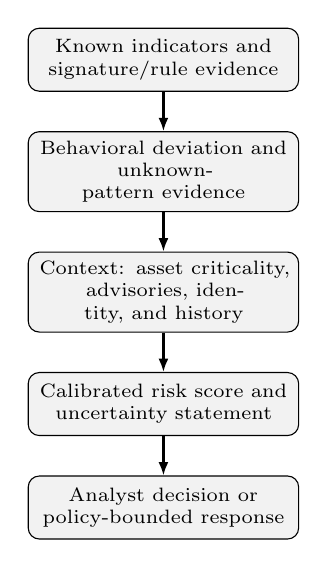
\begin{tikzpicture}[node distance=5mm, every node/.style={font=\scriptsize}, item/.style={draw, fill=gray!10, rounded corners, align=center, text width=32mm, minimum height=8mm}, arrow/.style={-{Latex[length=1.7mm]}, thick}]
\node[item] (known) {Known indicators and\\signature/rule evidence};
\node[item, below=of known] (behavior) {Behavioral deviation and\\unknown-pattern evidence};
\node[item, below=of behavior] (context) {Context: asset criticality,\\advisories, identity, and history};
\node[item, below=of context] (risk) {Calibrated risk score and\\uncertainty statement};
\node[item, below=of risk] (decision) {Analyst decision or\\policy-bounded response};
\draw[arrow] (known) -- (behavior);
\draw[arrow] (behavior) -- (context);
\draw[arrow] (context) -- (risk);
\draw[arrow] (risk) -- (decision);
\end{tikzpicture}
\caption{Threat-analysis evidence path. Each stage adds context; feedback and model monitoring are applied after the response decision.}
\label{fig:evidencepath}
\end{figure}

\begin{figure*}[!t]
\centering
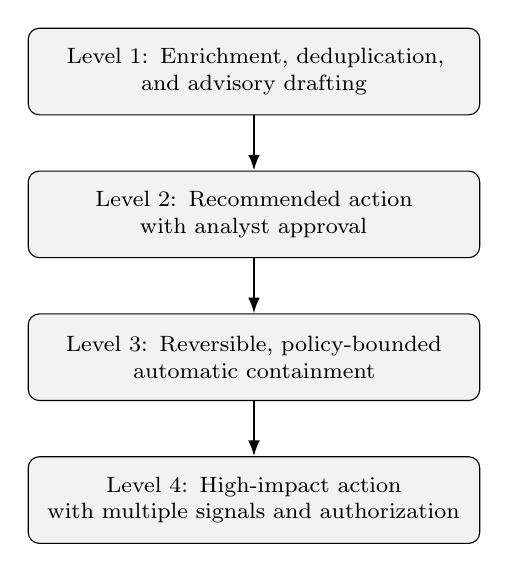
\begin{tikzpicture}[node distance=7mm, every node/.style={font=\footnotesize}, level/.style={draw, fill=gray!10, rounded corners, align=center, minimum height=11mm, text width=55mm}, arrow/.style={-{Latex[length=2mm]}, thick}]
\node[level] (assist) {Level 1: Enrichment, deduplication,\\and advisory drafting};
\node[level, below=of assist] (recommend) {Level 2: Recommended action\\with analyst approval};
\node[level, below=of recommend] (bounded) {Level 3: Reversible, policy-bounded\\automatic containment};
\node[level, below=of bounded] (critical) {Level 4: High-impact action\\with multiple signals and authorization};
\draw[arrow] (assist.south) -- (recommend.north);
\draw[arrow] (recommend.south) -- (bounded.north);
\draw[arrow] (bounded.south) -- (critical.north);
\end{tikzpicture}
\caption{Graduated autonomy model for AI-assisted incident response. Increasing autonomy requires stronger evidence, authorization, reversibility, and audit controls at every level.}
\label{fig:autonomy}
\end{figure*}

\section{Explainability, Generative AI, and RAG}
\subsection{Explainable AI}
Security decisions are consequential: an unexplained alert may be ignored, while an unexplained containment action may interrupt critical services. Explainability can be local, global, example-based, feature-based, or causal. LIME explains an individual classifier prediction with a local interpretable approximation and remains a widely used baseline \cite{Ribeiro2016}. A useful security explanation should identify evidence, time window, entities, confidence or uncertainty, and the counterfactual or missing evidence that would change the decision.

The supplied GNN/LLM study combines graph models and LIME to make file-threat predictions more accessible \cite{Balaji2025}. A readable explanation may describe local model behavior without proving causal validity. Explanations should therefore be evaluated for faithfulness, stability, analyst usefulness, and manipulation resistance. A dashboard exposing source records and detector-level scores can complement model explanations and reduce overreliance on generated narratives.

\subsection{LLMs and Security Advisory Systems}
LLMs can assist with alert summarization, report drafting, query translation, threat-intelligence extraction, and analyst dialogue. The supplied advisory study proposes tailoring reports from threat feeds and RSS sources to organizational requirements \cite{Abeywardena2023}. The conversational-advisor thesis explores domain-tuned open models with parameter-efficient adaptation and highlights domain knowledge, transparency, privacy, provider dependence, and computational cost \cite{Zhivonitko2026}. CyLens extends this idea to agentic threat intelligence and reports a system using a very large threat-report collection \cite{Liu2025}.

These systems should remain analyst-support tools unless actions are bounded by independent controls. LLMs may hallucinate indicators, misread technical language, leak sensitive context, follow malicious instructions in retrieved documents, or produce confident unsupported recommendations. A response system must separate observation, interpretation, recommendation, and execution. High-impact actions require policy checks, authorization, reversible steps, and human approval.

\subsection{RAG for Security Analysis}
RAG combines a generative model with a retriever and external evidence store. Lewis \emph{et al.} describe RAG as combining parametric and non-parametric memory, improving access to updateable knowledge and enabling provenance-oriented generation \cite{Lewis2020}. In security, a RAG system can retrieve vulnerability advisories, asset inventories, incident procedures, ATT\&CK descriptions, prior cases, and organizational policies before producing an advisory.

RAG is not automatically trustworthy. Retrieval can return stale, poisoned, irrelevant, or adversarial content. Security RAG needs source authenticity, access control, timestamps, chunk-level citations, retrieval evaluation, prompt-injection defenses, and output validation. A strong design shows original evidence beside every recommendation, labels uncertainty, and refuses execution when evidence is insufficient. The supplied advisory and observatory studies motivate this evidence-centered workflow \cite{Kaufhold2022,Abeywardena2023,Liu2025}.

\section{Automated Response and SOC Assistance}
Detection and response should be evaluated as a closed operational loop rather than isolated classification. A SOC assistant can normalize events, correlate entities, enrich alerts, estimate risk, recommend containment, draft an advisory, and record analyst feedback. The Observatory emphasizes modular sources, filtering, interrelations, assessment, integration, and export for CERT work \cite{Kaufhold2022}. Schmitt and Koutroumpis argue that AI security measures should be combined with policy interventions and continuous adaptation to address systemic and autonomous-AI risks \cite{Schmitt2025}.

Automation should be graduated by confidence and reversibility. Low-risk enrichment, deduplication, and report drafting can be automated more readily than endpoint isolation, account disablement, or destructive remediation. Every automated action should have a reason, evidence links, policy authorization, rollback path, audit record, and escalation route. The literature supports AI assistance and workflow automation, but does not justify unrestricted autonomous response.

\section{Comparative Analysis and Research Gaps}
Table~\ref{tab:comparison} compares supplied and external studies. The literature is rich in proposed models and focused evaluations but less consistent in external validation, temporal testing, operational cost, and response safety.
\begin{table*}[t]
\caption{Comparative Analysis of Selected Studies}
\label{tab:comparison}\centering\scriptsize
\begin{tabularx}{\textwidth}{c c Y Y Y Y Y}\toprule
Ref. & Year & Approach & Model or method & Dataset/evaluation & Key contribution & Limitation\\\midrule
\cite{Kaufhold2022} & 2022 & CERT observatory & Design science dashboard & 12 expert walkthrough/interviews & Situational awareness and integration requirements & Not a detection benchmark\\
\cite{Manoharan2022} & 2022 & AI/ML review & ML, DL, NLP overview & Literature and case discussion & Broad taxonomy & Empirical details limited\\
\cite{Abeywardena2023} & 2023 & SOC advisory & Threat feeds, RSS, NLP dashboard & Proposal; metrics not reported & Tailored advisory workflow & Validation limited\\
\cite{Rajendran2024} & 2024 & Deep anomaly detection & CNN and RNN & Dataset not reported in abstract & Deep model comparison & Setup and generalization unclear\\
\cite{KumarBhatRisk} & 2025 & Risk assessment & XGBoost, RF, SVM, LR, autoencoder & Security bulletins; metrics reported & Text, CVSS, classification, novelty & Scope and drift limited\\
\cite{Balaji2025} & 2025 & Explainable detection & GCN, LSH, LIME, LLM & Uploaded files; setup limited & Relational detection and explanations & Robustness open\\
\cite{Liu2025} & 2025 & Agentic CTI & LLM plus NLP modules & 271,570 reports; comparative evaluation & CTI lifecycle assistance & Agent safety open\\
\cite{Zhivonitko2026} & 2026 & Conversational advisor & LoRA-tuned open models & Curated QA; automatic metrics & Domain-tuned assistance & Thesis-scale evidence\\
\cite{SommerPaxson} & 2010 & NIDS critique & ML methodology & Closed-world analysis & Generalization concerns & Foundational study\\
\cite{Mirsky2018} & 2018 & Online anomaly detection & Autoencoder ensemble & Network streams/testbed & Streaming architecture & Environment-specific\\
\cite{Arp2022} & 2022 & ML methodology & Pitfall analysis & 30 papers plus experiments & Evaluation recommendations & Adoption remains open\\
\cite{Lewis2020} & 2020 & RAG & Retriever plus generator & NLP tasks & External, updateable evidence & Security threats not addressed\\
\bottomrule\end{tabularx}\end{table*}

\begin{figure}[!t]
\centering
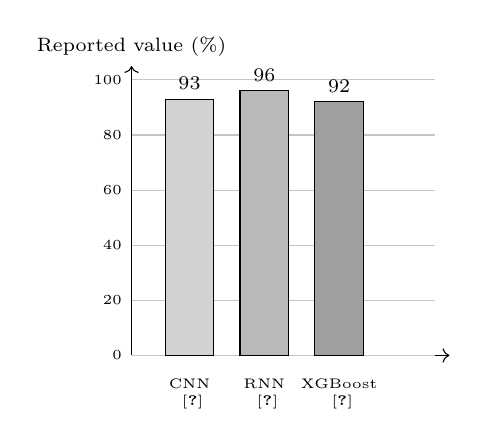
\begin{tikzpicture}[x=0.95cm,y=0.035cm]
\draw[->] (0,0) -- (0,105) node[above, font=\scriptsize]{Reported value (\%)};
\draw[->] (0,0) -- (4.25,0);
\foreach \y in {0,20,40,60,80,100} {
	\draw[gray!45] (0,\y) -- (4.05,\y);
	\node[left, font=\tiny] at (0,\y) {\y};
}
\draw[fill=gray!35] (0.45,0) rectangle (1.10,93);
\draw[fill=gray!55] (1.45,0) rectangle (2.10,96);
\draw[fill=gray!75] (2.45,0) rectangle (3.10,92);
\node[above, font=\scriptsize] at (0.775,93) {93};
\node[above, font=\scriptsize] at (1.775,96) {96};
\node[above, font=\scriptsize] at (2.775,92) {92};
\node[below, align=center, text width=16mm, font=\tiny] at (0.775,-5) {CNN\\\cite{Rajendran2024}};
\node[below, align=center, text width=16mm, font=\tiny] at (1.775,-5) {RNN\\\cite{Rajendran2024}};
\node[below, align=center, text width=18mm, font=\tiny] at (2.775,-5) {XGBoost\\\cite{KumarBhatRisk}};
\end{tikzpicture}
\caption{Selected performance values reported by two supplied studies. The values use different tasks, datasets, and experimental settings; they are not a cross-study ranking.}
\label{fig:reportedmetrics}
\end{figure}

\subsection{Evidence-Based Gaps}
\textbf{G1: Longitudinal and cross-environment validation.} The closed-world problem, benchmark limitations, and documented ML pitfalls \cite{SommerPaxson,Tavallaee2009,Arp2022} are reinforced by supplied studies that report focused experiments without consistent external validation \cite{Rajendran2024,KumarBhatRisk,Balaji2025}. Research should evaluate temporal splits, organization transfer, and concept drift.

\textbf{G2: Calibrated hybrid decisions.} The supplied literature separately discusses signatures, anomaly detection, threat intelligence, dashboards, and advisory generation \cite{Kaufhold2022,KumarBhatRisk,KumarBhatTemporal,Abeywardena2023}. A gap remains in principled fusion with calibrated uncertainty, cost-sensitive thresholds, and analyst feedback.

\textbf{G3: Operationally faithful explainability.} LIME and GNN explanations are promising \cite{Ribeiro2016,Balaji2025}, but faithfulness, stability, analyst usefulness, and manipulation resistance are not evaluated uniformly. Future work should measure whether explanations improve correct triage rather than merely readability.

\textbf{G4: Safe generative automation.} RAG offers updateable evidence and provenance potential \cite{Lewis2020}, while supplied studies motivate LLM advisory and agentic CTI workflows \cite{Abeywardena2023,Liu2025,Zhivonitko2026}. Missing evidence concerns prompt injection, poisoned intelligence, hallucination, privacy, authorization, rollback, and the boundary between recommendation and execution.

\textbf{G5: Reproducible real-time evaluation.} Online detection and operational dashboards address streaming and analyst needs \cite{Mirsky2018,Kaufhold2022}, but studies do not consistently report end-to-end latency, throughput, resource cost, alert fatigue, or response reliability. Shared streaming benchmarks with realistic benign workloads and changing attack distributions are needed.

\section{Future Research Directions}
Future systems should be evaluated as evidence-preserving, adaptive decision pipelines. Datasets should be temporally ordered, documented, and tested across environments, with explicit treatment of label delay, class imbalance, and benign rare events. Hybrid models should expose detector provenance and calibrate risk rather than equating anomaly with maliciousness. Robustness evaluation should include evasion, poisoning, adversarial examples, and corrupted telemetry; adversarial machine learning is a persistent security concern \cite{BiggioRoli}.

XAI should be evaluated with technical and human measures: fidelity, stability, comprehensibility, time to triage, and error detection by analysts. RAG and LLM systems should use authenticated sources, timestamped retrieval, least-privilege access, prompt isolation, structured outputs, and independent policy validators. Automated response should use graduated autonomy, simulation or shadow mode before enforcement, reversible actions, and explicit human escalation. Studies should report computational cost, privacy protections, and reproducible artifacts.

These directions motivate a possible SecureX-style framework combining signatures, rules, ML anomaly analysis, real-time monitoring, risk assessment, an evidence-grounded advisor, and controlled response. This is a research direction inferred from the gaps, not a claim that SecureX has achieved any reported performance.

\section{Conclusion}
Taken together, the literature points to a layered form of AI-driven cybersecurity rather than a single replacement technology. Signatures and rules remain the most practical foundation for known threats and auditable control. Machine learning and deep learning can widen coverage to behavioral and anomalous patterns, but only when their data, temporal testing, calibration, and drift are treated seriously. Dashboards and advisory tools address the human bottleneck that raw detection scores leave untouched. XAI is useful when it exposes faithful evidence, not merely a persuasive explanation, and LLMs or RAG systems are valuable only when their sources, permissions, and recommendations can be checked. The most credible direction is therefore a partnership between deterministic controls, adaptive models, analysts, and carefully bounded automation.

\begin{thebibliography}{99}
\bibitem{Kaufhold2022} M.-A. Kaufhold, A. S. Basyurt, K. Eyilmez, M. Stöttinger, and C. Reuter, ``Cyber threat observatory: Design and evaluation of an interactive dashboard for computer emergency response teams,'' in \emph{Proc. 30th Eur. Conf. Inf. Syst. (ECIS)}, 2022.
\bibitem{Manoharan2022} A. Manoharan and M. Sarker, ``Revolutionizing cybersecurity: Unleashing the power of artificial intelligence and machine learning for next-generation threat detection,'' \emph{Int. Res. J. Modernization Eng. Technol. Sci.}, vol. 4, no. 12, 2022, doi: 10.56726/IRJMETS32644.
\bibitem{Abeywardena2023} K. Abeywardena, T. A. D. L. P. T. Arachchi, C. Y. S. Nanayakkara, J. M. I. P. Jayaweera, and D. R. B. Dissanayake, ``Automating threat advisory report generation using threat intelligence,'' in \emph{Proc. 2023 Int. Conf. Innovative Comput., Intell. Commun. Smart Elect. Syst. (ICSES)}, 2023, doi: 10.1109/ICSES60034.2023.10465533.
\bibitem{Ismail2024} W. S. Ismail, ``Threat detection and response using AI and NLP in cybersecurity,'' \emph{J. Information Systems and Informatics}, 2024.
\bibitem{Rajendran2024} T. Rajendran, J. K., M. I. N., and B. Sampathkumar, ``Cybersecurity threat detection using deep learning and anomaly detection techniques,'' in \emph{Proc. 2024 Int. Conf. Knowledge Eng. Commun. Syst. (ICKECS)}, 2024, doi: 10.1109/ICKECS61492.2024.10617347.
\bibitem{KumarBhatRisk} S. Kumar and C. R. Bhat, ``Enhancing cybersecurity risk assessment with text mining of security bulletins and advisory data,'' manuscript, 2025.
\bibitem{Balaji2025} V. S. Balaji, R. M. Charles, A. G. P. S., D. J. E., S. K., and V. P., ``Explainable AI-driven cyber threat detection using graph neural networks and large language models for interpretability and contextual analysis,'' in \emph{Proc. 2nd Int. Conf. Comput. Data Sci. (ICCDS)}, 2025, doi: 10.1109/ICCDS64403.2025.11209348.
\bibitem{Schmitt2025} M. Schmitt and P. Koutroumpis, ``Cyber shadows: Neutralizing security threats with AI and targeted policy measures,'' \emph{IEEE Trans. Artif. Intell.}, vol. 6, no. 7, 2025, doi: 10.1109/TAI.2025.3527398.
\bibitem{Liu2025} X. Liu, J. Liang, Q. Yan, J. Jang, S. Mao, M. Ye, J. Jia, and Z. Xi, ``CyLens: Towards reinventing cyber threat intelligence in the paradigm of agentic large language models,'' arXiv:2502.20791v2, 2025.
\bibitem{Zhivonitko2026} M. Zhivonitko, ``Designing a conversational cyber threat advisor using domain-tuned conversational AI,'' bachelor's thesis, Oulu Univ. Appl. Sci., Finland, 2026.
\bibitem{KumarBhatTemporal} S. Kumar and C. R. Bhat, ``A temporal-aware cyber threat intelligence model for predicting emerging attacks from sequential security advisories,'' in \emph{Proc. 4th Int. Conf. Inventive Comput. Informatics (ICICI)}, 2026, doi: 10.1109/ICICI68773.2026.11581276.
\bibitem{SommerPaxson} R. Sommer and V. Paxson, ``Outside the closed world: On using machine learning for network intrusion detection,'' in \emph{Proc. IEEE Symp. Security and Privacy}, 2010, pp. 305--316, doi: 10.1109/SP.2010.25.
\bibitem{BuczakGuven} A. L. Buczak and E. Guven, ``A survey of data mining and machine learning methods for cyber security intrusion detection,'' \emph{IEEE Commun. Surveys Tuts.}, vol. 18, no. 2, pp. 1153--1176, 2016, doi: 10.1109/COMST.2015.2494502.
\bibitem{Shone2018} N. Shone, T. N. Ngoc, V. D. Phai, and Q. Shi, ``A deep learning approach to network intrusion detection,'' \emph{IEEE Trans. Emerg. Topics Comput. Intell.}, vol. 2, no. 1, pp. 41--50, 2018, doi: 10.1109/TETCI.2017.2772792.
\bibitem{Mirsky2018} Y. Mirsky, T. Doitshman, Y. Elovici, and A. Shabtai, ``Kitsune: An ensemble of autoencoders for online network intrusion detection,'' in \emph{Proc. NDSS}, 2018, doi: 10.14722/ndss.2018.23204.
\bibitem{Moustafa2015} N. Moustafa and J. Slay, ``UNSW-NB15: A comprehensive data set for network intrusion detection systems,'' in \emph{Proc. Mil. Commun. Inf. Syst. Conf. (MilCIS)}, 2015, pp. 1--6, doi: 10.1109/MILCOM.2015.7357948.
\bibitem{Tavallaee2009} M. Tavallaee, E. Bagheri, W. Lu, and A. A. Ghorbani, ``A detailed analysis of the KDD CUP 99 data set,'' in \emph{Proc. IEEE Symp. Comput. Intell. Security Defense Appl.}, 2009, pp. 1--6, doi: 10.1109/CISDA.2009.5356528.
\bibitem{Liao2013} H.-J. Liao, C.-H. R. Lin, Y.-C. Lin, and K.-Y. Tung, ``Intrusion detection system: A comprehensive review,'' \emph{J. Netw. Comput. Appl.}, vol. 36, no. 1, pp. 16--24, 2013, doi: 10.1016/j.jnca.2012.09.004.
\bibitem{Ribeiro2016} M. T. Ribeiro, S. Singh, and C. Guestrin, ``Why should I trust you?: Explaining the predictions of any classifier,'' in \emph{Proc. 22nd ACM SIGKDD Int. Conf. Knowledge Discovery Data Mining}, 2016, pp. 1135--1144, doi: 10.1145/2939672.2939778.
\bibitem{BiggioRoli} B. Biggio and F. Roli, ``Wild patterns: Ten years after the rise of adversarial machine learning,'' \emph{Pattern Recognit.}, vol. 84, pp. 317--331, 2018, doi: 10.1016/j.patcog.2018.07.023.
\bibitem{Lewis2020} P. Lewis, E. Perez, A. Piktus, F. Petroni, V. Karpukhin, N. Goyal, H. Küttler, M. Lewis, W.-t. Yih, T. Rocktäschel, S. Riedel, and D. Kiela, ``Retrieval-augmented generation for knowledge-intensive NLP tasks,'' in \emph{Adv. Neural Inf. Process. Syst.}, vol. 33, 2020.
\bibitem{Arp2022} D. Arp, E. Quiring, F. Pendlebury, A. Warnecke, F. Pierazzi, C. Wressnegger, L. Cavallaro, and K. Rieck, ``Dos and don'ts of machine learning in computer security,'' in \emph{Proc. 31st USENIX Security Symp.}, 2022.
\end{thebibliography}
\end{document}
